\chapter{Implemetace a testování}
\label{sec:implementace}
Tato kapitola se bude zabývat popisem implementace nástroje pro tvorbu FMEA. Na základě daných skutečností popsaných v předchozí kapitole byla vytvořena webová aplikace. Základní rozdělení této aplikace je na front-end(klientská část) a back-end(serverová část) . Ač je tato aplikace postavena převážně na straně klienta, tak bude následující popis obsahovat i kapitolu pro popis serverové části.

\section{Backend}
Požadavků, které se v této aplikaci zpracovávají na straně serveru není mnoho. Nicméně to k k čemu se serverová část využívá by se dalo zúžit na dvě oblasti: 
\begin{itemize}
    \item Ukládání a načítání analýzy
    \item Sdílení dat mezi uživateli
\end{itemize}

\subsection{Ukládání a načítání analýzy}
Pro persistentní uložení dat analýzy se používá MongoDB, kde je objekt analýzy uložen v nezměněném stavu jako součást uloženého dokumentu. Struktura objektu obsahující data nalýzy je součástí přílohy(\ref{src:data}) této diplomové práce. Struktura obsahuje zejména základní atributy pro ukázku zanořenosti objektu, některé méně důležité atributy jsou zjednodušeny nebo vynechány. Toto ukládání je provedeno pouze na základě vyvolané události od uživatele. Zároveň platí, že pro persistentní ukládání dat analýzy musí být uživatel přihlášen. V opačném případě mu nejsou tyto možnosti zobrazeny v rámci menu. Toto platí i z toho důvodu, že každý záznam databáze je přiřazen určitému uživateli. Přihlášený uživatel si poté může načítat své uložené analýzy. Pro manipulaci s databází je použit ODM framework Mongoose, v rámci kterého je potřeba definovat model ukládaných dokumentů. Tento model obsahuje tyto parametry: 
\begin{itemize}
    \item \textbf{ID} - Unikátní identifikační číslo dokumentu. Pro vytvoření tohoto čísla se používá knihovna uuidv4 \cite{uuid}, která generuje náhodný 36-místný unikátní řetězec znáků složených z písmen a-z a číslic 0-9.  
    \item \textbf{data} - Objekt, který obsahuje všechna potřebná data analýzy v původním formátu.
    \item \textbf{ownerID} - Identifikační číslo přihlášeného uživatele. Toto číslo má každý registrovaný uživatel v rámci platformy Firebase, která se používá pro práci s uživatelskými účty a bude popsána později. 
\end{itemize}

Pro připojení k databázi se používá metoda \textit{mongoose.connect(connectionString)}, jejímž parametrem je řetězec obsahující odkaz na databázový server a případně údaje k uživatelskému účtu v rámci MongoDB. Tyto údaje nejsou součástí zdrojového kódu, ale jsou získány na základě tzv. proměnných prostředí. Pro manipulaci dokumentů se pak používají asynchroní metody, které lze zavolat na objekt vytvořený v rámci modelu. Tyto metody jsou: 
    
\begin{itemize}
    \item \textit{create(object)} - Tato metoda se používá pro vytvoření dokumentu v rámci modelu pro analýzu. Tato metoda přijímá jako parametr objekt, jehož atributy, byly definovány v předchozím výčtu. 
    \item \textit{findOne(object)} - Metoda pro nalezení jednoho dokumentu v kolekci dokumentů. Metoda přijímá objekt, jehož atributem je nejčastěji pouze id hledaného dokumentu. 
    \item \textit{find(object)} - Pomocí této metody lze nalézt v kolekci dokumentu jeden a více dokumentů. Parametrem je objekt obsahující, v tomto případě, identifikační číslo uživatele.   
    \item \textit{deleteOne(object)} - Tato metoda slouží pro smazání jednoho dokumentu v kolekci na základě poskytnutého id, které je atributem objektu v parametru metody. 
    \item Zvláštností ze strany použitého ODM je, že neposkytuje uspokojivé řešení pro aktualizaci dokumentu. Jediná možnost, která funguje pro aktualizaci je použití metod, které dokážou například přidat jeden atribut k dokumentu. Bohužel nebyl nalezen jednoduchý způsob nebo metoda, jak aktualizovat celý dokument jako takový. Což je vlastnost, která je v rámci vyvůjeného nástroje žádoucí. Změny totiž postihují často několik atributů objektu analýzy. Řešení bylo nakonec použití kombinace metody pro smazání a vytvoření nového aktualizovaného záznamu, což je způsob účinný, ale ne zrovna efektivní.  
\end{itemize}

\subsection{Sdílení dat mezi uživateli}
Další zajímavější oblastí, která je řešena na straně serveru je sdílení dat mezi uživateli v reálném čase. Je to jedna z hlavních funkcí, na které je aplikace postavena umožňující efektivní práci týmu provádějící analýzu. Tuto funkcionalitu zajišťuje knihovna Socket.IO. 

Socket.IO je knihovna, která umoňuje rychlou, obousměrnou komunikaci mezi klientem a serverm založenou na eventech. \cite{socketIO} Tato knihovna je postavena na komunikačním protokolu WebSocket, což je protokol umoňující navázání a udržení komunikace mezi klientem a serverem. Socket.IO také využívá pro realizaci metod GET(získání dat ze serveru) a POST(odeslání dat na server) tzv. HTTP long-polling. Jedná se o alternativní metodu, která byla využívána v dobách, kdy prohlížeče komunikaci přes protokol WebSocket nepodporovali. Velikou výhodou obou těchto metod je, že nabízí alternativu oproti standardní komunikaci mezi klientem a serverem, kdy je navázáno spojení, vytvořen požadavek, odeslání odpovědi a ukončení spojení. V tomto případě lze po navázání spojení vytvářet několik požadavků bez ztráty spojení.

Další výhodou oproti samotnému použití řešení používající pouze protkol WebSocker je, že Socket.IO nabízí řešení pro některé základní problémy, které se řeší při sdílení dat mezi uživateli. Příkladem je rozdělení uživatelů do skupin na základě ID a broadcast prováděných změn mezi ostatní účastníky skupiny. Příklad takovéhoto rozdělení je vidět na obrázku \ref{fig:rooms}. 

\begin{figure}[h]
\centering
	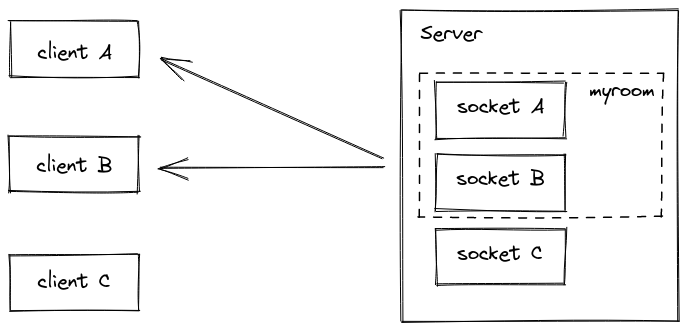
\includegraphics[width=1.0\textwidth]{Figures/rooms.png}
	\caption{Skupiny v rámci Socket.IO}
	\label{fig:rooms}
\end{figure}

Co se týká implementace této komunikace na straně serveru, tak se úvodem inicializuje server použitím metody z knihovny \uv{socket-io} \  s parametry číslo portu a volitelným objektem, který se používá pro zamezení chyby CORS, která nastává v případě přístupu k adrese z jiné domény. Dále se pracuje s událostmi a to tím způsobem, že klient vytváří různé typy událostí a server naopak čeká na několik typů těchto události a patřičně na ně reaguje. Zde je seznam událostí, se kterými se pracuje v rámci komunikace mezi klientem a serverem: 

\begin{itemize}
    \item \textbf{connection} - Inicializační událost, která informuje server o připojení nového uživatele.
    \item \textbf{get-analysis} - Tato událost je vyvolána pro první načtení dat analýzy. Parametrem této metody je vygenerované nové ID, které je obsaženo v url odkazu, a které se dále použije jako ID vytvořené místnosti připojených uživatelů. Uživatel, který vyvolal událost \textbf{connection} je přidán do skupiny s tímto ID pomocí metody \textit{join} poskytované knihovnou. 
    \item \textbf{send-changes} - Další událost se pak již stará o sdílení změn provedených uživateli. Server reaguje na tuto událost rozesláním přijatých dat v rámci vyvolání vlastní události \textbf{receive-changes}, na jejíž zpracování zase čeká klient. Tato událost je zaslána všem uživatelům v rámci skupiny kromě uživatele, který vyvolal původní událost. 
    \item \textbf{save-analysis} - Další událost se již týká práce s dokumenty v databázi. První událost je reakce na žádost uživatele pro uložení nové analýzy. Data analýzy jsou parametrem události.  
    \item \textbf{update-analysis} - Další se pak stará již o aktualizaci existujícího dokumentu metodou popsanou v předchozí kapitole. Data jsou zde také součástí parametru události. 
      \item \textbf{load-analysis} - Poslední metoda slouží pro načtení všech uložených analýz uživatelem. Parametrem této události je ID uživatele. Server jako reakci na tuto událost vyvolá vlastní událost \textbf{receive-analyses} obsahující kolekci načtených dat. 
\end{itemize}

Implementace na straně klienta je taková, že se použije metoda io z knihovny \uv{socket.io-client}, která má jako parametr url adresu serveru. Metoda vrácí objekt, který se pak používá ve všech komponentách, které mění data aplikace. Pomocí tohto objektu se pak vyvolávají a zachycují výše uvedené události. 



\section{Frontend}
V této kapitole bude ukázána hlavní část aplikace a to klientská část, se kterou interaguje uživatel přístupující k webové aplikaci. Postupně budou popsány jednotlivé části aplikace jak z uživatelského tak implementačního úhlu pohledu. 

\subsection{Struktura aplikace}
Jak již bylo zmíněno v kapitole \ref{subsection:react}, tak při použití Reactu vývojář tvoří strukturu aplikace pomocí komponent. Na obráku \ref{fig:structure} je vidět hlavní stránka aplikace rozdělena do těchto komponent. Zde je výčet těchto komponent rozlišených v rámci obrázku barevnými obdelníky odpovídající barvě textu: 

\begin{itemize}
    \item \textcolor{blue}{App} - Hlavní komponenta aplikace, která obsahuje všechny ostatní viditelné komponenty. Komponenta je pouze součástí komponent, které jsou zodpovědné za směrování url odkazů a komponenta v rámci balíčku React-redux, což je knihovna, která slouží pro správu globálního stavu dat aplikace a bude popsána později.  
    \item \textcolor{green}{Navigation} - Komponenta, která vystupuje v aplikaci jako menu. Toto menu je víceúrovňové a obsahuje položky pro manipulaci s dokemntem analýzy, dále popdpůrné funkce při tvorbě analýzy a napravo sekci pro registraci a přihlášení k uživatelskému účtu. 
    \item \textcolor{red}{Header} - Tato komponenta obsahuje první krok analýzy a to hlavičku obsahující základní informace o analýze. Údaje se zadávají do textových polí, které disponují animací, která při kliknutí popisný text zobrazí na vrchní stranu elementu a umožní zadávání textových hodnot. Při zadání alespoň jedné hodnoty v rámci hlavičky zůstavají elementy ve stavu pro zadávání textu.  
    \item \textbf{TreeGraph} - Jedná se o jednu z hlavních komponent aplikace, která slouží pro grafické zobrazení náhledu analýzy. Jak je vidět, tak lze v rámci této komponenty tvořit stromovou strukturu analyzovaného produktu. Součástí komponety je i ukazatel rozsahu přiblížení nacházející se na spodní straně komponenty. Detailněji bude tato komponenta popsána v kapitole \ref{sec:grafika} zaměřené na grafický náhled aplikace. 
    \item Následují komponety sloužící jako textový náhled na analýzu. Ač se může zdát, že tabulkový náhled tvoří jeden tabulkový element, tak při tomto zobrazení to není úplně možné. Proto je tabulka rozdělena na komponety \textcolor{pink}{VerticalTable} a \textcolor{magenta}{HorizontalTable}. \textcolor{pink}{VerticalTable} obsahuje první dva kroky analýzy: strukturální a fuknční analýzu. \textcolor{magenta}{HorizontalTable} pak obsahuje analýzu selhání a rizik a optimalizační kroky. Jak je vidět tak v rámci kroků analýzy, kde se mezi atributy tvoří relace, tak jsou tyto vztahy správně reprezentovány i v tabulce pomocí slučování řádků tabulky. Proto, že se obsah analýzy může roztáhnout na větší prostor než je možné zobrazit v rámci šířky a výšky okna, tak lze zobrazená část tabulky měnit pomocí posuvníků. Díky těmto možnostem manipulace se zobrazením obsahu spolu s funkcemi pro zobrazení obsahu v rámci grafického režimu se aplikace jeví i jako docela responzivní a lze ji celkem bez problému zobrazit na zařízeních s různým rozlišením obrazovky. 

\end{itemize}

\begin{figure}[t]
\centering
	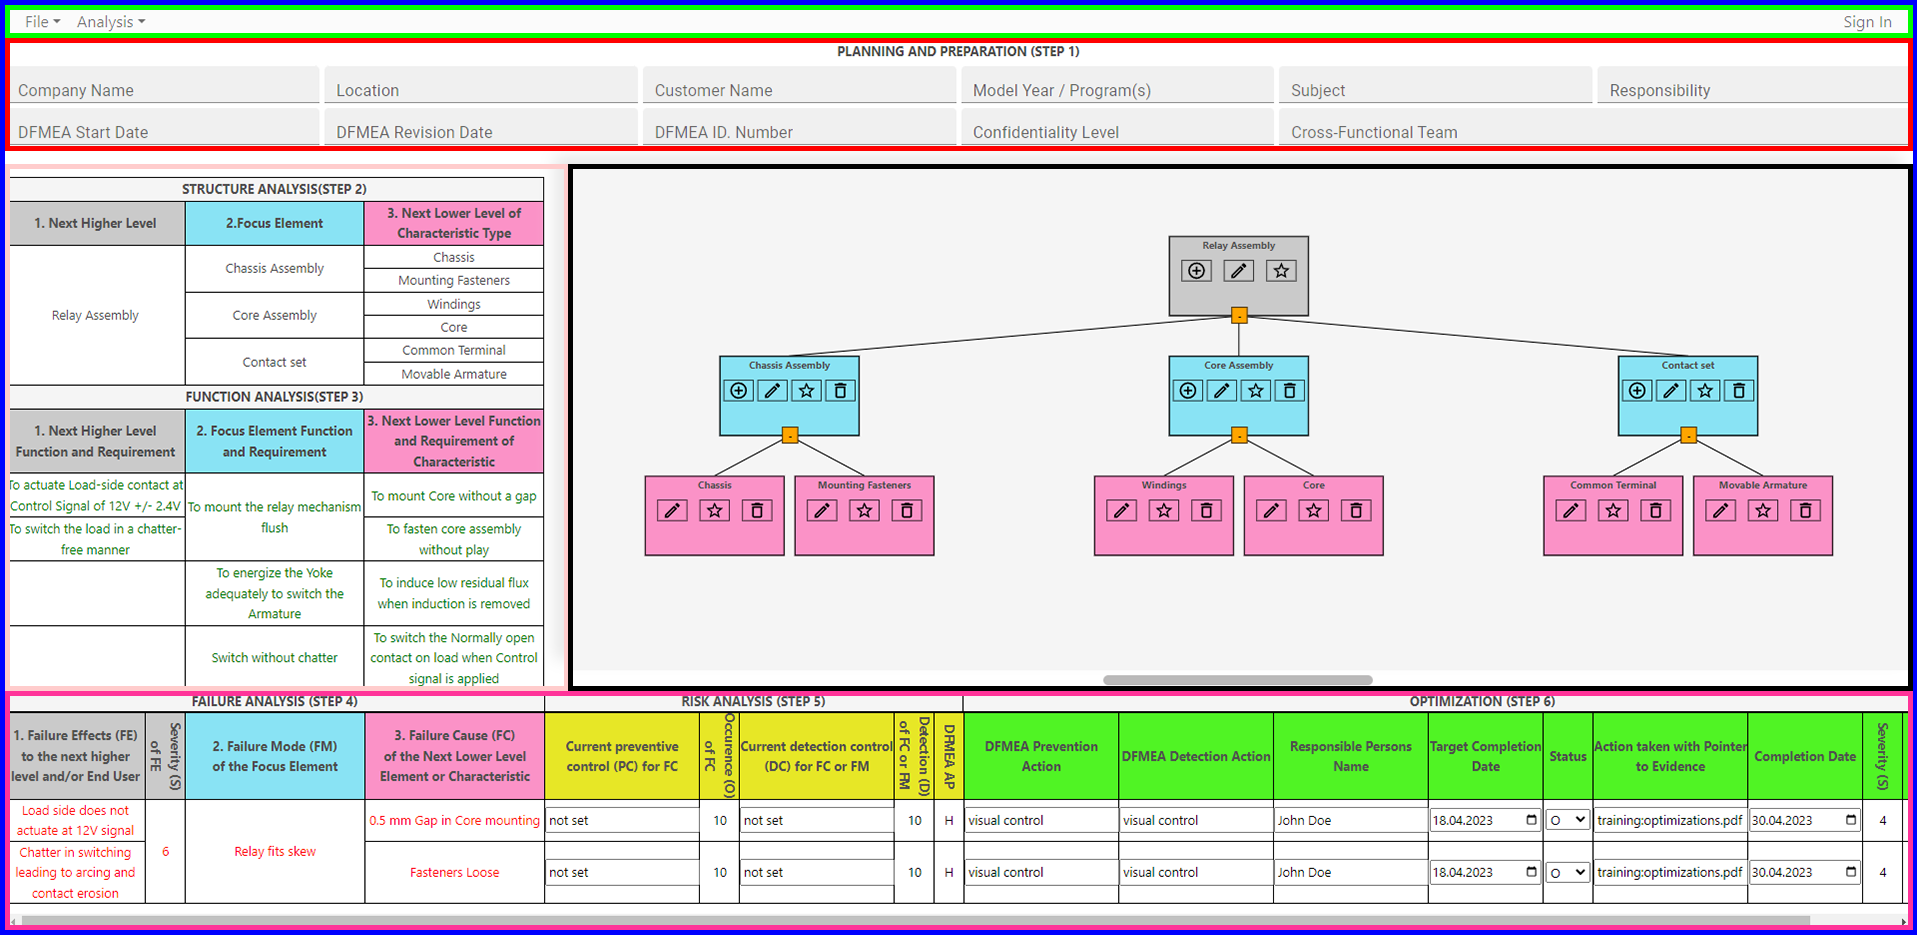
\includegraphics[width=1.0\textwidth]{Figures/componenty2P.png}
	\caption{Struktura aplikace}
	\label{fig:structure}
\end{figure}

\begin{itemize}
    \item Poslední důležitou komponentou je \textcolor{orange}{Modal}, která je zobrazena na obrázku \ref{fig:modal}. Modal umožňuje používat aplikaci jednoduše bez přecházení na jiné podstránky aplikace. Modal je tzv. modální okno, které se zobrazuje jakoby na nové vsrtvě stránky. Vyvolání zobrazení tohoto modálního okna je možné zpravidla kliknutím na tlačítko nebo položku v menu. Podle elementu, který vyvolal zobrazení modálního okna se zobrazí i odpovídající obsah. Modal může například sloužit pro úpravu objektů v rámci grafického náhledu, zobrazení tabulky pro hodnocení rizik, registrace a přihlášení k uživatelskému účtu apod. Zavření modálního okna je provedeno kliknutím kdekoli mimo okno nebo stisknutí klávesy Escape. 
\end{itemize}
\begin{figure}[t]
\centering
	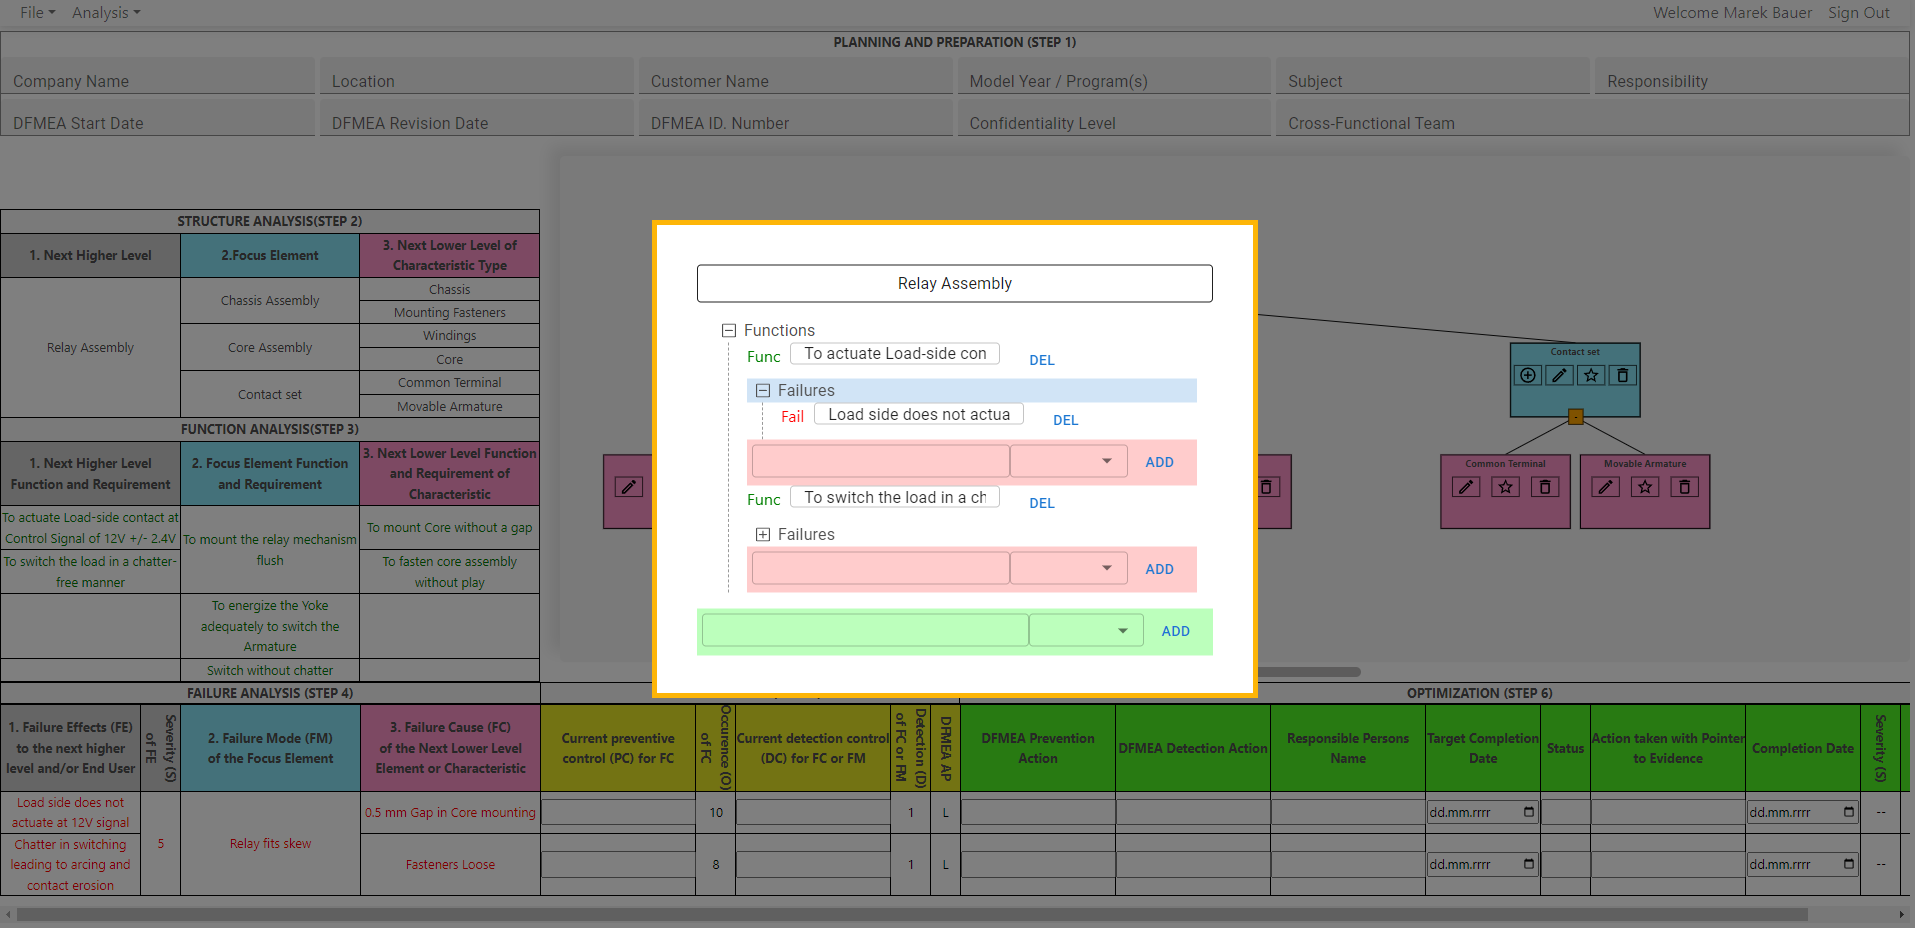
\includegraphics[width=1.0\textwidth]{Figures/modalP.png}
	\caption{Modální okno(komponenta)}
	\label{fig:modal}
\end{figure}

\newpage
\subsection{Tvorba analýzy}
Začátek tvorby analýzy se provádí vybráním typu analýzy zaměřené na návrh nebo proces. Na základě této volby se upráví několik několik hlaviček tabulky, které slouží pro detailnější popis toho, co se má vyplňovat. Dále se také upraví hodnotící tabulky, které obsahují slovní reprezentaci stupnice pro určení hodnotících atributů. Všech šest tabulek pro hodnocení se v rámci obou typů liší a to jak obsahem, tak bohužel i počtem sloupců a strukturou. Z toho důvodu nebylo možné při implementaci uložit tyto data do stejné datové struktury a dále je jednotným způsobem zpracovat a zobrazit, ale bylo potřeba jednotlivé zobrazení a data vytvořit manuálně. 

Následuje první krok analýzy a to vyplňení hlavičky se základními údaji o analýze. V této části by bylo dobré zmínit knihovnu, která se využívá na několika místech v rámci webové aplikace. Jméno této knihovny je Material UI \cite{mui}, která nabízí použití předem vytvořených komponent zejména v rámci formulářů a dalších funkčních prvků. Příkladem jsou textové vstupy v hlavičce dokumentu. Tyto textové vstupy jsou komponenty TextField importované z této knihovny s nastavením vlastních parametrů pro určení názvu, funkce zpracovávající události a také výběr z předem definových stylů. Další podstatné komponenty, které jsou použity v aplikaci: 
\begin{itemize}
    \item \textbf{Box} - Komponenta, která slouží jako zapouzdřující element obsahující další prvky. Obdoba HTML elementu div.
    \item \textbf{Modal} - Modal je komponenta popsaná již v předchozí kapitole zaměřené na popis struktury z pohledu komponent. Důležitou součástí této komponenty jsou parametry open a onClose, kterým je potřeba nastavit proměnnou a funkci, které určují, kdy je modal viditelný a jaká funkce se provede po vyvolání události pro zavření modalního okna.  
    \item \textbf{Button} - Tlačítko s předem daným stylem. Lze nastavit typ, variantu, formulář a metodu pro zpracování události při kliknutí. 
    \item \textbf{Treeview} - Tato komponenta je využita v rámci úpravy objektů v grafickém náhledu a slouží pro zobrazení stromové struktury funkcí a selhání podobně jako při zobrazení adresářové struktury v počítači. V rámci parametrů komponenty lze nastavit i vlastní ikony, které slouží pro rozbalení nebo zabalení odpovídajících položek. Jednotlivé položky v rámci stromové struktury jsou vlastně další komponenty z knihovny MaterialUI a to StyledTreeItem.
    \item \textbf{Autocomplete} - Tato komponenta slouží jako vstup ve formuláři, která obsahuje seznam položek, ze kterých je možné vybrat. Tento seznam je definován jako pole v rámci parametru komponenty. Konkrétně se používá při určování relací mezi funkcemi a selháními, kdy pro nově vytvářené funkce nebo selhání na první a třetí úrovni, je potřeba vybrat vybrat funkci nebo selhání z druhé úrovně. Obdobou je kombinace HTML elementů select a option. 
    \item \textbf{List} - List je komponenta sloužící pro jednoduché zobrazení seznamu položek. Obsahuje další pomocné komponenty pro definování hlavičky, položky seznamu, tlačítka a ikony. Je použita v rámci zobrazení a výběru uložených analýz uživatelem. 
    \item \textbf{Tabs} - Poslední uvedená komponenta slouží pro členění obsahu do přepínatelných záložek s různým obsahem. Obsahuje další komponenty Tab a TabPanel pro definování záložky a obsahu, který se má zobrazit při kliknutí na záložku. Je využita v rámci definování vlastních příkladů pro určování hodnotících atributů (Vážnost, Výskyt, Detekce) na počátku analýzy. 
\end{itemize}

Kromě těchto komponent je z knihovny použito několik volně dostupných ikon, které se vyskytují, jak součást komponent, tak samotně například pro vzhled tlačítek v rámci objektů v grafickém režimu. Tvorba analýzy dále pokračuje v rámci grafického a tabulkového náhledu na analýzu, který bude popsán v rámci samostatných kapitol.  

\subsubsection{Grafický náhled na analýzu}
\label{sec:grafika}
Grafický náhled slouží zároveň i pro tvorbu analýzy pro kroky: analýza struktury, funkcí a selhání. Náhled zajišťuje dříve zmíněná komponenta TreeGraph. Pro zobrazení stromové struktury objektů je použita knihovna React D3 Tree \cite{d3tree}. Tato knihovna je nadstavbou obsáhlé knihovny D3.js, která umožňuje zobrazení a manipulaci s grafickými objekty pomocí Javascriptu. Použitá knihovna umožňuje zobrazení stromové struktury objektů tím, že se v rámci importované komponenty Tree definuje jako parametr data, objekt s atributem children, což je pole dalších objektů na další úrovni stromu. Knihovna implicitně poskytuje některé funkce pro práci s tímto grafickým zobrazením jako je přibližování a oddalování zobrazeného obsahu, posouvání struktury tažením myší, zobrazení a skrytí prvků na další úrovní apod. Dále je také možné použít vlastní implementaci pro některé části řešení. Příkladem je nastavení vlastních čár spojující jednotlivé objekty nastavení parametru komponenty pathFunc nebo použití vlastních tvarů a obsahu jednotlivých objektů nastavením parametru renderCustomNodeElement.

Obě tyto možnosti byly při implementaci využity. První funkci bylo potřeba nastavit svg objekt, který znázorňuje přímku s počátečními a koncovými souřadnicemi x a y podle šířky objektu. Druhá možnost nastavení vlastních tvarů a obsahu objektů byla vyřešena vytvořením vlastních komponent, které obsahují jednak definovaný tvar, ale také název objektu a sadu nástrojů pro manipulaci s objekty. Detailní ukázku této komponenty je možné vidět na obrázku \ref{fig:node}. Komponeta obsahuje(seznam nástrojů je popsán z levé strany): 


\begin{figure}[h]
\centering
	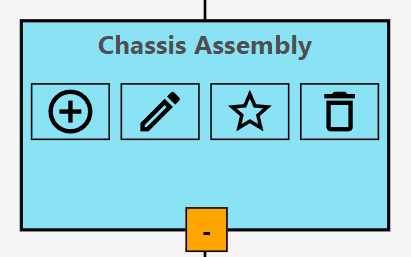
\includegraphics[width=0.7\textwidth]{Figures/node.png}
	\caption{Komponenta objektu v grafickém režimu}
	\label{fig:node}
\end{figure}


\begin{itemize}
    \item \textbf{Jméno objektu} - Název objektu v rámci stromové struktury. 
    \item \textbf{Přidat} - Pomocí tohoto tlačítka se přidává danému objektu další potomek. 
    \item \textbf{Upravit} - Toto tlačítko slouží pro zobrazení modálního okna, kde lze nastavit jméno objektu. Dále přidávat, editovat a mazat funkce a selhání, které odpovídají danému objektu ze strukturální analýzy. Objekt vždy obsahuje seznam funkcí a k tomu odpovídající seznam selhání, které je možné zobrazit nebo skrýt. Na konci těchto seznamů je vždy formulář, který slouží pro přidání nové funkce nebo selhání. Všechny zobrazené hodnoty jsou zobrazeny v textovém vstupu a jejich hodnota lze kdykoli upravit. Ukázka této funkce již bylo možné zhlédnout při popisu komponenty Modal na obrázku \ref{fig:modal}.
    \item \textbf{Označit} - Tlačítko, které nabízí jednu z dalších zajímavých funkcí aplikace. Pomocí kliknutí na toto tlačítko se označí objekt a všechny jeho přidružené funkce a selhání, reprezentované buňkami v tabulkovém zobrazení, oranžovou barvou. Díky tomu je v tabulce jednoznačně možné určit, které hodnoty mezi sebou navzájem souvisí. Tato funkce byla implementována jednoduchým polem identifikátorů, které se kontrolují při renderování tabulky. 
    \item \textbf{Smazat} - Poslední tlačítko v sadě nástrojů slouží pro odstranění objektu ze struktury. Úskalím při implementaci bylo tzv. kaskádové mazání. Při smazání objektu v rámci struktury je potřeba také smazat všechny jeho přidružené funkce a selhání, které se navíc v rámci zanořeného objektu vyskytují na více místech. 
    \item \textbf{Rozbalit/zabalit} - Poslední tlačítko již není v seznamu nástrojů, ale nachází se na spodní straně objektu. Slouží pro zobrazení nebo skrytí potomků daného objektu. 
\end{itemize}

K popisu těchto komponent ještě patří pravidlo, že kořenový objekt neobsahuje možnost pro jeho smazání a objekty na třetí úrovní neobsahují možnost pro přidávání dalších potomků. Je to z důvodu dané logiky strukturální analýzy. 

Jedno z implementačních rozhodnutí se týkalo volby orientace stromové struktury. Knihovna nabízí obě varianty, tedy zobrazení horizontální i vertikální. Nakonec bylo vybráno zobrazení horizontální z důvodu toho, že se struktura při tvorbě rozsrůstá spíše do šířky než do výšky a vzhledem k tomu jaké má komponenta pro grafické zobrazení míry, tak se toto rozhodnutí zdálo přívětivější. 


\subsubsection{Tabulkový náhled na analýzu}
Zobrazení analýzy pomocí textové tabulky je druhá varianta, která slouží pro tvorbu analýzy. Oproti grafickému režimu pak slouží k tvorbě analýzy rizik a případně stanovení optimalizačních opatření. Z implementačního pohledu bylo zobrazení některých dat docela náročné z důvodu správného zobrazení relací mezi atributy a odpovídajícího slučování buněk. Tabulkám bylo potřeba nastavit fixní layout a určit přímo šířku všech sloupců, aby tabulka neměnila velikost při zadávání různě dlouhého obsahu. V tabulkovém zobrazení se hodně pracuje s hlavním objektem, ve kterém jsou uložena všechna potřebná data. Běžný problém, který se řeší ve webových aplikací je to, aby měly všechny potřebné komponenty přístup ke stejným datům. Řešením tohoto problému je použití knihovny React-redux \cite{redux} , která slouží jako globální stav nějakých dat a umožňuje komponentám přístup k tomuto stavu a jeho modifikaci. Stavy se skládají z těchto čtyř souborů: 
\begin{itemize}
    \item \textbf{Reducer} - Hlavní soubor, který obsahuje inicializaci objektu s atributy, který slouží pro určení nějakého stavu. Dále obsahuje metodu, jejímiž atributy jsou state a action. Akce je objekt skládající se z parametrů type a payload. Na základě typu akce se pak provede příslušná modifikace stavu. V případě této knihovny je nutné vždy vracet nový objekt a ne pouze modifikovat aktuální. 
    \item \textbf{Typy} - Tento pomocný soubor obsahuje výčet všech typů akcí, které mohou v rámci daného stavu nastat. 
 \item \textbf{Akce} - Zde jsou obsaženy všechny akce, které mají komponenty k dispozici pro práci s daným stavem dat. V rámci komponent je potřeba použít speciální metodu \textit{useDispatch}, která vrací objekt umožňující vyvolání nějaké akce. Tyto akce pak zachytává a zpracovává reducer. 
 \item \textbf{Selektor} - Poslední soubor se používá se pro získání stavu dat. Selektor může obsahovat metody, které uložené data nějakým způsobem filtrují nebo modifikují a vrací požadovanou strukturu. 
\end{itemize}
V rámci zobrazení tabulky se používájí metody v rámci selektoru, které filtruje zejména definové funkce a selhání v rámci analýzy z hlavního objektu do pole. Pomocí tohoto pole je pak snažší zobrazit požadované relace při renderování buněk tabulky. 

Co se týká tvorby samotné tabulky tak je potřeba vyfiltrované data zobrazit odpovídajícím způsobem tak, aby byly dodrženy všchechny požadované relace. Pro průchod daty jsou použity cykly, které postupně tvoří textový řetězec, který je následně převeden do reprezentace HTML elementů. Horizontální tabulka také obsahuje sadu formulářových vstupů jako je tlačítko pro zobrazení modálního okna, textový vstup, výběr ze seznamu nebo výběr datumu.


\subsubsection{Podpůrné funkce}
Tyto funkce slouží pro zjednodušení tvorby analýzy tím, že poskytují nastavení vstupních hodnot, zaznamenávaní aktivit při setkání týmu a výstup z analýzy. Zde je seznam těchto funkcí a jejich krátky popis:
\begin{itemize}
    \item \textbf{Nastavení vlastních příkladů pro určení hodnotících atributů} - Tato funkce slouží pro nastavení clastních příkladů v rámci atributů Vážnost, Výskyt a Detekce. Tato činnost by se měla provést před začátkem vypracování samotné analýzy. Nastavení se provádí v rámci modálního okna, které obsahuje pro všechny tři atributy deset textových vstupů, kde je možné definovat slovní hodnocení rizik. Toto hodnocení se pak zobrazuje v příslušných tabulkách hodnotících atributů. 
    \item \textbf{Tvorba zápisu ze setkání týmu} - Další funkce slouží pro zaznamenávání aktivit z jednotlivých sektání týmu. Jedná se vlastně o tabulku s atributy: ID, Datum, Popis, Související dokumenty a Aktualizováno. Zápisy jsou zobrazeny v tabulce, pod kterou se nachází formulář pro přidání nového zápisu. 
 \item \textbf{Kontrola úplnosti analýzy a výsledky} - Tato funkce slouží zejména pro závěrečnou fázi analýzy. Jak je vidět na obrázku \ref{fig:results}, tak funkce zobrazí graf obsahující rozdělení všech rizik do tří hodnot AP(Low, Medium, High), zároveň jsou rizika dělena na počáteční a koncová. Na základě těchto dvou hodnot je také možné zobrazené slouce filtrovat, kliknutím na popis dané hodnoty na horní straně grafu. Tato i všechny ostatní funkce jsou součástí knihovny Chart.js \cite{chart}, která byla použita pro zobrazení grafu. 
 Pod grafem se nachází tabulka, která ve zjednodušeé formě obsahuje všechna nalezená rizika. Zároveň je zde kontrola, že všechny rizika jsou v jednom z konečných stavů, tedy optimalizována nebo určena, že není potřeba optimalizovat. Stav pro určení rizika, které nepotřebuje optimalizaci lze určit kliknutím na políčko v tabulce. Změna tohoto stavu má za následek, že i zbytek řádku tabulky pro optimalizaci daného rizika je znepřístupněn a nelze psát do formulářových vstupů hodnoty. 
\end{itemize}

Na závěr popisu tvorby analýzy je ještě dobré dodat, že aplikace na několika místech obsahuje informační vysvětlivky. Příkladem je práce s objekty v grafickém režimu. Pro práci s objekty se používají tlačítka s ikonami, které při najetí myši zobrazí krátkou vysvětlivku o činnosti daného tlačítka. Druhým příkladem je zobrazení dodatečné informace při najetí na hodnotu AP v rámci tabulkového náhledu. V tomto případě se zobrazí informace o hodnotě RPN na základě, které byla určena hodnota AP. 
\begin{figure}[h]
\centering
	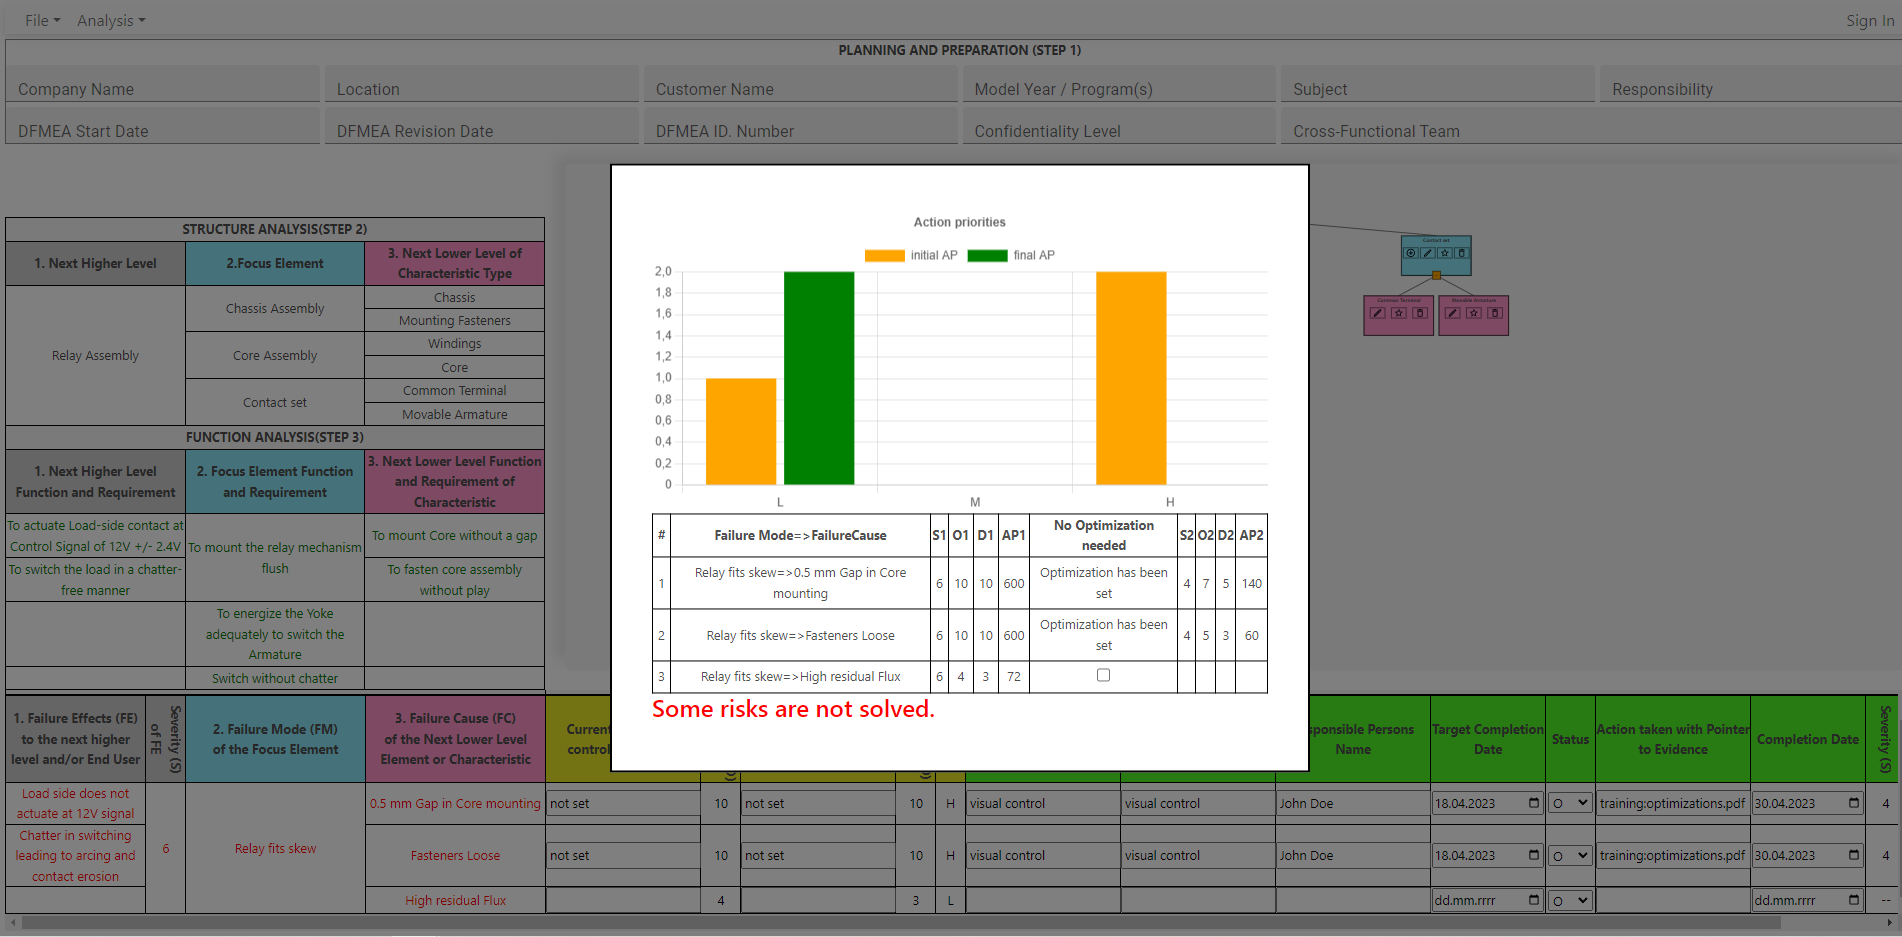
\includegraphics[width=1.0\textwidth]{Figures/results.png}
	\caption{Zobrazení výsledků analýzy}
	\label{fig:results}
\end{figure}

\newpage
\subsection{Správa uživatelkých účtů}
Nástroj nabízí základní možnosti pro přihlášení k uživatelskému účtu. Účet slouží pro zpřístupnění funkcí pro ukládání a načítaní analýzy z databáze. Formulář pro přihlašování je také vyřešen pomocí modálního okna(obr. \ref{fig:sign}). Možnosti přihlášení jsou dvě: 
\begin{itemize}
    \item \textbf{Pomocí vlastního účtu} - Pomocí této možnosti je nutné se nejdříve registrovat zadáním uživatelského jména, emailu a hesla.  
    \item \textbf{Pomocí Google účtu} - Druhá možnost nabízí přihlášení k účtu uživatelskému účtu pomocí již vytvořeného účtu v rámci aplikace Google.
\end{itemize}

\begin{figure}[t]
\centering
	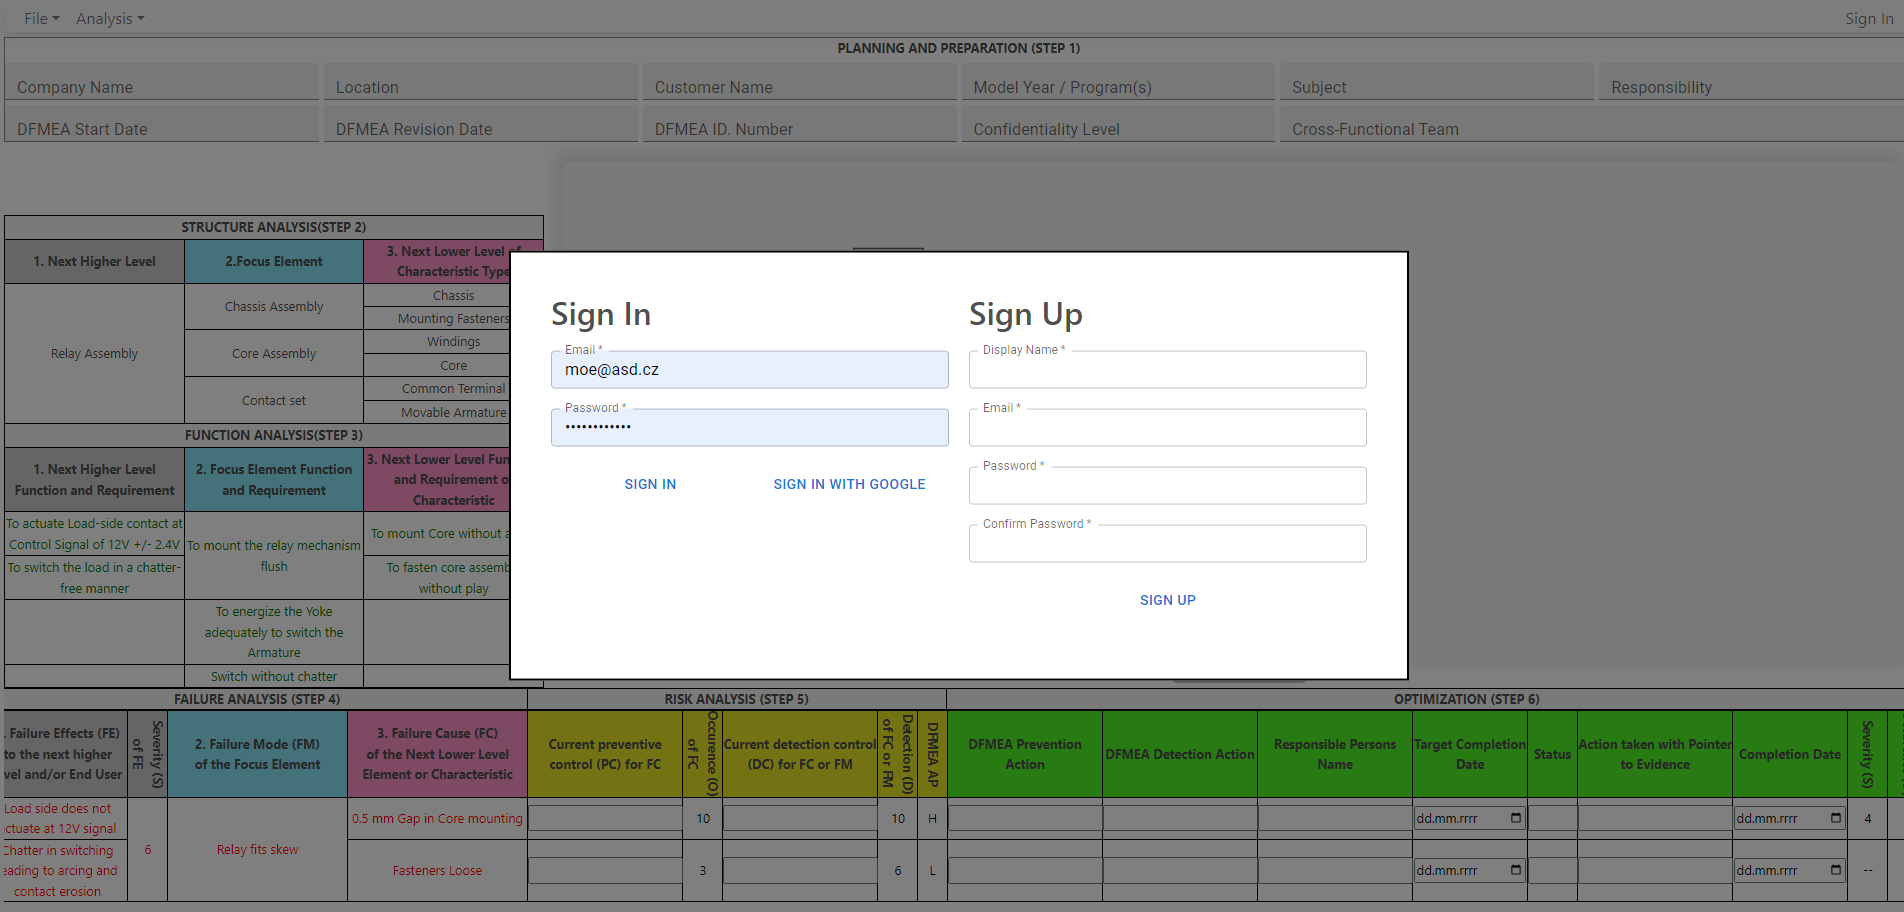
\includegraphics[width=1.0\textwidth]{Figures/sign.png}
	\caption{Přihlašování k uživatelskému účtu}
	\label{fig:sign}
\end{figure}

Obě tyto možnosti poskytuje platforma pro vývoj webových aplikací Firebase \cite{firebase}. Po založení vlastního účtu na této platformě je možné využít jejich nástroj k autentizaci, kde lze povolit přihlašování pomocí různých možností. Platforma poskytuje vlastní API, pomocí kterého lze využívat metody při implementaci. Prvním krokem je incializace aplikace pomocí konfigurančních údajů, které jsou součástí účtu. Dále lze využít například metody \textit{singInWithGooglePopup}, která slouží pro vyvolání pop-up okna s možností přihlášení ke Google účtu. Další velice zajímavou nabízenou funkcí je poskytnutí metody, která funguje na principu návrhového vzoru observer. V kombinaci s ukládáním stavu o uživateli pomocí React-redux knihovny lze reagovat na změny stavu o přihlášeném uživateli. 

V rámci správy uživatelů je také vytvořena jednoduchá funkce pomocí, které lze automaticky kopírovat odkaz na aktuální analýzu do schránky. Odkaz má tento formát: doména/analyses/\uv{unikátníID}. O zkopírování adresy do schránky je uživatel informován jednoduchým pop-up oknem, který vystupuje v aplikaci jako samotatná komponenta a může být využita pro sdělení různých krátkých informací.  


\subsection{Export a import}
Poslední uvedenou funkcí nástroje je export a import částí analýzy do různých formátů. V rámci této funkce si tak může uživatel načítat a ukládat data jako soubory na své zařízení. Základní funkcí je export a import dat analýzy do formátu JSON. Díky této možnosti si může uživatel uložit stav své analýzy do tohoto souboru a kdykoliv jej načíst zpět. Při importu dat ze souboru se provádí základní ověření správnosti formátu. Konkrétně je v aplikaci vytvořena datová struktura Map, která má formát klíč-hodnota. Klíčem jsou všechny atributy, které může objekt obsahovat a hodnota je jejich datový typ. Pokud má importovaný objekt atributy, které neodpovídají dané mapě, tak není objekt importován. 

V rámci grafického režimu je vytvořena stromová struktura, kterou lze také exportovat do formátu PNG. Pro vytvoření tohoto obrázku bylo potřeba modifikovat danou strukturu, tak aby zbytečně neobsahovala nástroje pro modifikaci objektů. Zde je také vidět výhoda komponent a to jejich znovupoužitelnost. V aplikaci se tak vyskytuje komponenta s grafem ve dvou verzích, kdy jedna obasahuje objekty s upraveným vzhledem pro export. Obsah této komponety je pak stáhnut pomocí balíčku react-component-export-image \cite{exportIMG}. Výsledek je možné vidět na obrázku \ref{fig:graphPNG}.

\begin{figure}[h]
\centering
	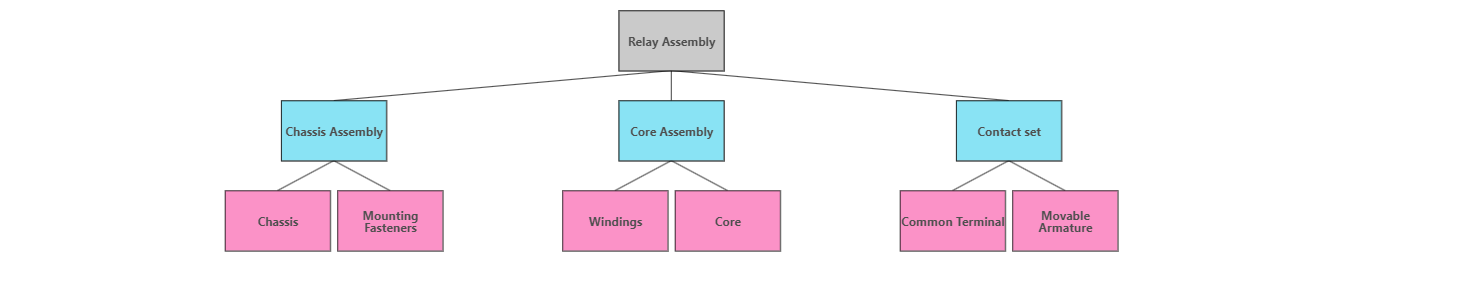
\includegraphics[width=1.0\textwidth]{Figures/Relay_Assembly.png}
	\caption{Export struktury do formátu PNG}
	\label{fig:graphPNG}
\end{figure}

Poslední funkcí pro export je možnost stáhnout celý tabulkový náhled na analýzu do formátu XLS, který lze otevřít například pomocí tabulkového editoru Microsoft Excell. Pro tuto funkci byl použit balíček react-export-table-to-excel \cite{exportTable}, který obsahuje metodu pro export dokonce více tabelkových elementů, které jsou v rámci jednoho obalujícího elementu. Problém při použití této nebo jiné knihovny, že i zde bylo potřeba upravit tabulku pro export. Jednak musela být použit složitější způsob renderování tabulky a slučování buněk a také v některých částí tabulky bylo potřeba nahradit prvky formulářů jejich hodnotami. Toho bylo docíleno rekurzivní funkcí, která postupně procházela potomky tabulkového elementu a při nálezu formulářového vstupu je nahradila jejich hodnotou. Výstřižek ze zobrazení pomocí tabulkového editoru je vidět na obráku  \ref{fig:excel} . 

\begin{figure}[h]
\centering
	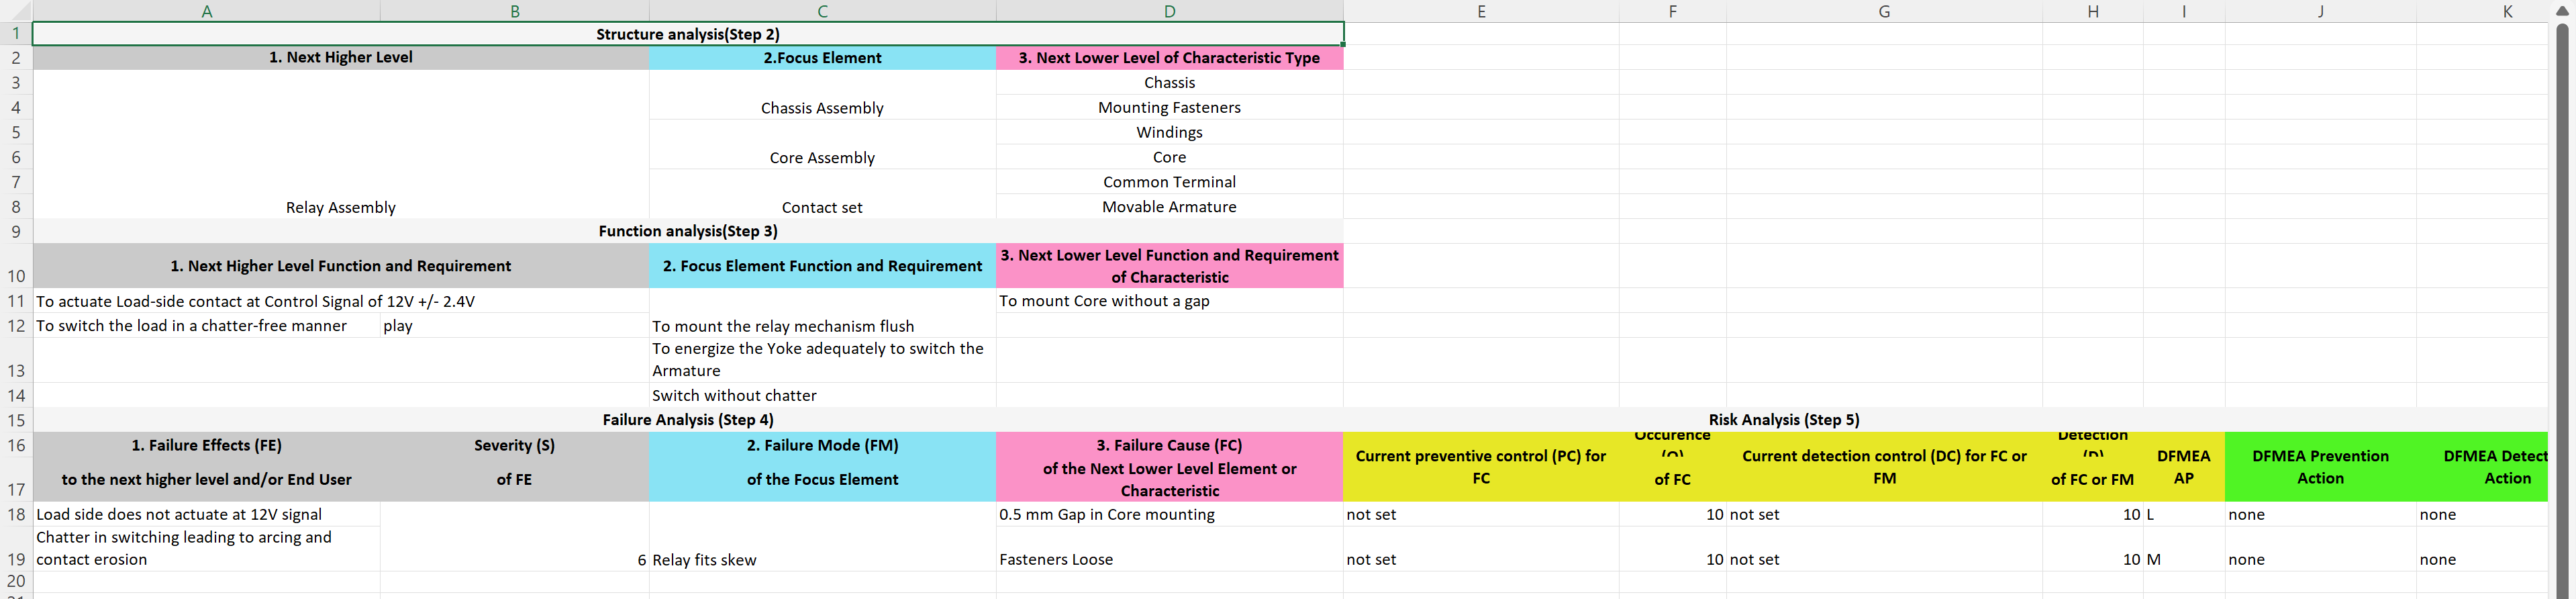
\includegraphics[width=1.0\textwidth]{Figures/excel.png}
	\caption{Export tabulky do formátu XLS}
	\label{fig:excel}
\end{figure}

Výhodou těchto exportů je, že si uživatel může dodatečně upravit a přípapdně vytisknout jednotlivé části analýzy. U všech těchto exportů je nastavno jméno souboru podle kořenového objektu v rámci analýzy struktury. 

\section{Testování}
Pro testování aplikace byly zvoleny systémové testy, nebo-li testy, které mají za cíl ověřit funkčnost jednotlivých případů užití. Systémové testování se provádí jako jedno z posledních před samotným nasazením aplikace do produkce. Pro toto testování se v praxi využívají dva způsoby. První způsob je projít jednotlivé scénáře manuálně se snahou nalézt případné nedokonalosti. Druhý způsob je použití automatizovaných testů, které simulují chování uživatele. V rámci této diplomové práce byl nakonec zvolen způsob manuálního otestování aplikace dvěma nezávislými osobami. Důvodů pro toto rozhodnutí je více. Například v praxi by měl být tento způsob testování bežnější. Automatizované testy jsou v tomto případě zbytečně nákladné a ne tolik efektivní a hodí se spíše provádět automatizované testování komponent nebo integrační testy, které ověřují správnou provázanost komponent. Proto jsou ve firmách lidé, kteří procházejí jednotlivé případy užití samostatně a vytvoří zprávu, kde zhodnotí daný průchod scénářem. Další výhodou tohoto přístupu je, že test provádí jiná osoba než ta, která vytvořila danou aplikaci. V případě psaní testu vývojařem může dojít k přehlednutí akcí, které by jiný uživatel udělal jinak. 

Pro testování nástroje pro tvorbu FMEA byly osloveni dva kolegové, kterým byl dán přístup k produkční verzi aplikace pomocí repozitáře na GitHubu. O jednoduché spuštění aplikace pomocí jednoho příkazu se stará program Docker. Popis instalace nástroje je součástí přílohy \ref{sec:docker}. Dále byly vytvořeny tři případy užití, které pokrývají značnou část funkcionality nástroje. Tyto případy užití jsou součástí přílohy \ref{sec:UC}. Pro hodnocení testů byl také vytvořen jednoduchý formulář obsahující otázky ke každému testovacímu případu. 

\subsection{Zhodnocení provedených testů}
Formulář, který měli oslovení kolegové vyplňovat se skládal z otázky, jestli se podařilo naplnit účel v rámci každého případu užití. Dále také měli možnost vyplňit vlasními slovy připomínky, nedokonalosti, návrhy na zlepšení, na které při provádění daného testu narazily. Shrnutí těchto odpovědí jsou zobrazeny v tabulce \ref{tab:testovani}. 

Jak je vidět tak se podařilo projít všemi testovacími případy bez větších potíží. Některé připomínky pramenily z nekompletních znalostí problematiky FMEA, které by v praxi neměli být velkým problémem, kdy se počítá, že bude tým provádějící analýzu dostatečně obeznámem s jejími aspekty. Nicméně připomínky pro zpřehlednění a úpravu některých částí UI byly brány v potaz a třeba v případě vyplňování atributu Status byl nahrazen textový vstup výběrem možností ze seznamu. Většina nalezených problémů byla také dodatečně opravena. 

Toto testování mělo za cíl zjistit, jestli byl zvolen správný přístup při návrhu aplikace, tak aby uživatel přistupující k aplikaci, dokázal provádět zadané úkony. Jednotlivé případy užití byly definovány obecně bez konkrétních zadání na, co by měl uživatel kliknout apod. I přes to se těmto dvěma uživatelům bez hlubších znalostí dané problematiky podařilo projít danými případy bez větších potíží. Dalším cílem bylo také objevit možné nedokonalosti a chyby, které se vyskytly při procházení jinými subjekty.  


\begin{table}[h]
	\caption{Výskedky testování}
	\label{tab:testovani}
\begin{tabular}{|p{3cm} | p{6cm} | p{6cm} |}
\hline
 & \textbf{Tester \#1} & \textbf{Tester \#2} \\ \hline
 \multicolumn{3}{|c|}{\textbf{UC1: Tvorba FMEA}} \\\hline
\textbf{Podařilo se \break naplnit účel}? & ANO & ANO\\ \hline
\textbf{Připomínky} & Lepší popis prvků UI v grafickém režimu(label, placeholder,...). & Více prostoru pro zobrazení textu v rámci tabulkového režimu(např. atribut Status). \\ \hline
 \multicolumn{3}{|c|}{\textbf{UC2: Přihlášení k uživatelskému účtu}} \\\hline
\textbf{Podařilo se \break naplnit účel}? & ANO & ANO\\ \hline
\textbf{Připomínky} & Zlepšit validační hlášky při registraci.  &  \\ \hline

 \multicolumn{3}{|c|}{\textbf{UC3: Ukládán\&Načítání analýzy}} \\\hline
\textbf{Podařilo se \break naplnit účel}? & ANO & ANO\\ \hline
\textbf{Připomínky} & 
\begin{enumerate}

    \item  Občasné problémy s uložením nové analýzy.(Krok č.1)
    \item  Při přepnutí uživatelského účtu by se mohla vytvořit nová analýza.
    \item  Přidat možnost pojmenování analýzy při ukládání.
    \item  Problém s importem analýzy ze souboru v kombinaci s načtením analýzy z databáze.

\end{enumerate}
  &  
  
  \begin{enumerate}
    \item  Ukládání pouze pomocí jednoho tlačíka, které buď vytvoří nový záznam analýzy nebo uloží aktualizuje již uložený.
    \item  Zlepšit popis okna pro načítání analýz. (například pomocí tabulky s atributy)

\end{enumerate} 
\\ \hline

\end{tabular}\  
\end{table}

